\chapter{对抗搜索}

\section{对抗搜索}

\subsection{对抗搜索(Adversarial Search)}

在一些复杂的博弈论(Game Theory)问题中,每一轮操作都可能有许多决策,于是就会形成一棵庞大的博弈树。针对这样的问题可以使用对抗搜索,也被称为博弈搜索(Game Search),即在一个竞争的环境中,多个agents之间通过竞争获取利益。\\

多个agents在同一个搜索空间中搜索解决方案的情况,通常发生在游戏中。每个agent是其它agent的对手并且彼此竞争,因此每个agent都需要考虑其它agent的操作及该操作所产生的影响。对抗搜索的目标就是选择一个能够使收益最大化的策略。\\

\subsection{零和游戏(Zero-Sum Game)}

零和游戏意味着游戏双方有着相反的目标,换句话说,在游戏的任何终结状态下,所有玩家获得的总和等于零。例如井字棋(Tic-Tac-Toe)、象棋(chess)、围棋(Go)等都是零和游戏。\\

零和游戏是AI最常研究的游戏,这类游戏通常有两个玩家(称为MAX和MIN)轮流行动,游戏是具有完整信息和确定的。\\

这类游戏可以被形式化为:

\begin{itemize}
    \item $ s_0 $:初始状态
    \item $ ToMove(s) $:在状态$ s $下能够行动的玩家
    \item $ Actions(s) $:在状态$ s $下合法行动的集合
    \item $ Result(s, a) $:在状态$ s $下执行行动$ a $后的结果
    \item $ IsTermial(s) $:判断游戏是否结束
    \item $ Utility(s, p) $:玩家$ p $在终结状态$ s $的效用
\end{itemize}

例如对于井字棋游戏,MAX下X,MIN下O。初始状态$ s_0 $为一个$ 3 \times 3 $的空棋盘。\\

对于某个状态$ s_1 $:

\begin{figure}[H]
    \centering
    \begin{tabular}{|c|c|c|c|}
        \hline
                   & \textbf{1} & \textbf{2} & \textbf{3} \\
        \hline
        \textbf{1} & X          & O          & X          \\
        \hline
        \textbf{2} &            & O          & O          \\
        \hline
        \textbf{3} &            & X          &            \\
        \hline
    \end{tabular}
\end{figure}

$ Actions(s_1) = \{(x, (2,1)),\ (x, (3,1),\ (x, (3,3)))\} $。\\

如果MAX在$ (2, 1) $下X,可表示为$ Result(s_1, (x, (2,1)))$:

\begin{figure}[H]
    \centering
    \begin{tabular}{|c|c|c|c|}
        \hline
                   & \textbf{1} & \textbf{2} & \textbf{3} \\
        \hline
        \textbf{1} & X          & O          & X          \\
        \hline
        \textbf{2} & X          & O          & O          \\
        \hline
        \textbf{3} &            & X          &            \\
        \hline
    \end{tabular}
\end{figure}

对于某个最终状态$ s_2 $:

\begin{figure}[H]
    \centering
    \begin{tabular}{|c|c|c|c|}
        \hline
                   & \textbf{1} & \textbf{2} & \textbf{3} \\
        \hline
        \textbf{1} & X          & O          & X          \\
        \hline
        \textbf{2} & X          & O          & O          \\
        \hline
        \textbf{3} & X          & X          & O          \\
        \hline
    \end{tabular}
\end{figure}

MAX和MIN的效用函数分别表示:

\begin{itemize}
    \item $ Utility(s_2, MAX) = +1 $
    \item $ Utility(s_2, MIN) = -1 $
\end{itemize}

\newpage

\section{Minimax}

\subsection{博弈树(Game Tree)}

博弈树可以表示两名游戏参与者之间的一场博弈,他们交替行棋,试图获胜。树中的每一个结点都对应于棋盘的一种布局。\\

\begin{figure}[H]
    \centering
    \begin{forest}
        TTT/.style args={#1:#2}{
        make tab/.expanded=\forestove{content},
        label={\pgfkeysvalueof{/forest/label position #1}:$#2$}
        },
        TTT*/.style={
                make tab=::/::/::,
                content/.expand once=%
                \expandafter\vphantom\expandafter{\romannumeral-`0\forestov{content}},
                draw=none,
                append after command={(\tikzlastnode.north) edge (\tikzlastnode.south)},
                for descendants={before computing xy={l*=1.2}},
            },
        th/.style=thick,
        for tree={node options=draw, inner sep=+0pt, parent anchor=south, child anchor=north}
        %
        [
        X:O:X/:X:/O::O, TTT=r:
        [
        X:O:X/X:X:/O::O, TTT=r:
        [
        X:O:X/X:X:O/O::O, TTT=r:
        [
        X:O:X/X:X:O/O:X:O, TTT=b:0
        ]
        ]
        [
        X:O:X/X:X:/O:O:O, TTT=b:-1
        ]
        ]
        [
        X:O:X/:X:X/O::O, TTT=r:
        [
        X:O:X/O:X:X/O::O, TTT=r:
        [
        X:O:X/O:X:X/O:X:O, TTT=b:0
        ]
        ]
        [
        X:O:X/:X:X/O:O:O, TTT=b:-1
        ]
        ]
        [
        X:O:X/:X:/O:X:O, TTT=r:
        [
        X:O:X/O:X:/O:X:O, TTT=b:
        [
        X:O:X/O:X:X/O:X:O, TTT=b:0
        ]
        ]
        [
        X:O:X/:X:O/O:X:O, TTT=b:
        [
        X:O:X/X:X:O/O:X:O, TTT=b:0
        ]
        ]
        ]
        ]
    \end{forest}
\end{figure}

对于玩家MAX而言,他需要选择能够使效用函数最大化的行动。而对于玩家MIN而言,需要选择对MAX最不利的行动,即最小化MAX的效用(minimize maximum utility of MAX)。\\

\subsection{Minimax}

Minimax是一种递归算法,用于在博弈树中找到最优行动,其中MAX将选择最大化值,MIN将选择最小化值。算法执行深度优先搜索算法以探索完整的游戏树。\\

\begin{algorithm}[H]
    \caption{Minimax}
    \begin{algorithmic}[1]
        \Procedure{MinimaxSearch}{game, state} returns an action
        \State player = game.ToMove(state)
        \State value, move = MaxValue(game, state)
        \State \Return move
        \EndProcedure
        \\
        \Procedure{MaxValue}{game, state} returns a (utility, move) pair
        \If {game.IsTermial(state)}
        \State \Return game.Utility(state, player), null
        \EndIf
        \State v = $ - \infty $
        \For {a in game.Actions(state)}
        \State v2, a2 = MinValue(game, game.Result(state, a))
        \If {v2 > v}
        \State v, move = v2, a
        \EndIf
        \EndFor
        \State \Return v, move
        \EndProcedure
        \\
        \Procedure{MinValue}{game, state} returns a (utility, move) pair
        \If {game.IsTermial(state)}
        \State \Return game.Utility(state, player), null
        \EndIf
        \State v = $ + \infty $
        \For {a in game.Actions(state)}
        \State v2, a2 = MaxValue(game, game.Result(state, a))
        \If {v2 < v}
        \State v, move = v2, a
        \EndIf
        \EndFor
        \State \Return v, move
        \EndProcedure
    \end{algorithmic}
\end{algorithm}

例如有一个只有一个回合的游戏,MAX先进行行动:

\begin{figure}[H]
    \centering
    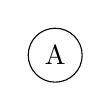
\begin{tikzpicture}[
            level distance=2cm,
            level 1/.style={sibling distance=5cm},
            level 2/.style={sibling distance=1.5cm},
            level 3/.style={sibling distance=1cm}
        ]
        \node[circle,draw] {A};
    \end{tikzpicture}
\end{figure}

MAX需要从当前状态$ A $中选择一个能使效用最大的行动。根据深度优先搜索的策略,首先选择$ A $的第一个子结点$ B $。\\

\begin{figure}[H]
    \centering
    \begin{tikzpicture}[
            level distance=2cm,
            level 1/.style={sibling distance=5cm},
            level 2/.style={sibling distance=1.5cm},
            level 3/.style={sibling distance=1cm}
        ]
        \node[circle,draw] {A}
        child {
                node[circle,draw] {B}
            }
        child {}
        child {};
    \end{tikzpicture}
\end{figure}

状态$ B $为MIN的回合,因此需要从$ B $中选择一个能使效用最小的行动。\\

\begin{figure}[H]
    \centering
    \begin{tikzpicture}[
            level distance=2cm,
            level 1/.style={sibling distance=5cm},
            level 2/.style={sibling distance=1.5cm},
            level 3/.style={sibling distance=1cm}
        ]
        \node[circle,draw] {A}
        child {
                node[circle,draw] (B) {B}
                child {node[circle,draw,fill=red] (E) {E}}
                child {node[circle,draw] (F) {F}}
                child {node[circle,draw] (G) {G}}
            }
        child {}
        child {};

        \node[above, yshift=0.5cm] at (B) {3};
        \node[below, yshift=-0.5cm] at (E) {3};
        \node[below, yshift=-0.5cm] at (F) {12};
        \node[below, yshift=-0.5cm] at (G) {8};
    \end{tikzpicture}
\end{figure}

同样,再从$ A $的剩余两个子结点$ C $和$ D $中,计算计算能使MIN效用最小的行动。\\

\begin{figure}[H]
    \centering
    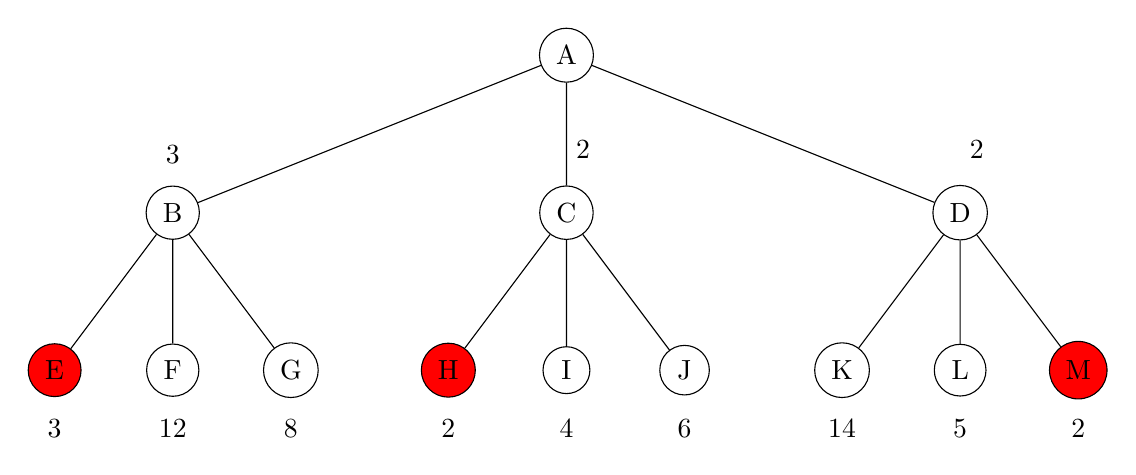
\begin{tikzpicture}[
            level distance=2cm,
            level 1/.style={sibling distance=5cm},
            level 2/.style={sibling distance=1.5cm},
            level 3/.style={sibling distance=1cm}
        ]
        \node[circle,draw] {A}
        child {
                node[circle,draw] (B) {B}
                child {node[circle,draw,fill=red] (E) {E}}
                child {node[circle,draw] (F) {F}}
                child {node[circle,draw] (G) {G}}
            }
        child {
                node[circle,draw] (C) {C}
                child {node[circle,draw,fill=red] (H) {H}}
                child {node[circle,draw] (I) {I}}
                child {node[circle,draw] (J) {J}}
            }
        child {
                node[circle,draw] (D) {D}
                child {node[circle,draw] (K) {K}}
                child {node[circle,draw] (L) {L}}
                child {node[circle,draw,fill=red] (M) {M}}
            };

        \node[above, yshift=0.5cm] at (B) {3};
        \node[below, yshift=-0.5cm] at (E) {3};
        \node[below, yshift=-0.5cm] at (F) {12};
        \node[below, yshift=-0.5cm] at (G) {8};

        \node[right, yshift=0.8cm] at (C) {2};
        \node[below, yshift=-0.5cm] at (H) {2};
        \node[below, yshift=-0.5cm] at (I) {4};
        \node[below, yshift=-0.5cm] at (J) {6};

        \node[right, yshift=0.8cm] at (D) {2};
        \node[below, yshift=-0.5cm] at (K) {14};
        \node[below, yshift=-0.5cm] at (L) {5};
        \node[below, yshift=-0.5cm] at (M) {2};
    \end{tikzpicture}
\end{figure}

最后,MAX从$ A $的三个子结点中选择一个能使效用最大的行动。\\

\begin{figure}[H]
    \centering
    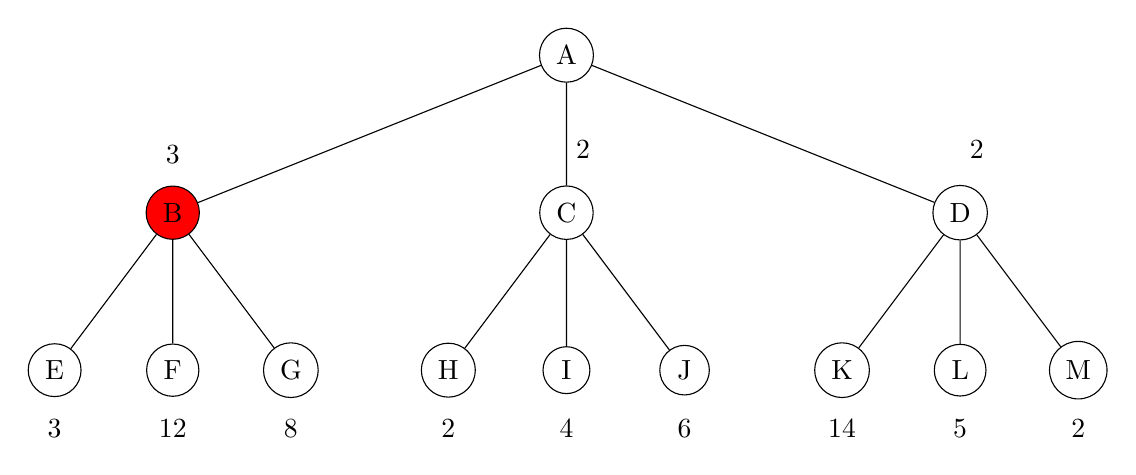
\begin{tikzpicture}[
            level distance=2cm,
            level 1/.style={sibling distance=5cm},
            level 2/.style={sibling distance=1.5cm},
            level 3/.style={sibling distance=1cm}
        ]
        \node[circle,draw] {A}
        child {
                node[circle,draw,fill=red] (B) {B}
                child {node[circle,draw] (E) {E}}
                child {node[circle,draw] (F) {F}}
                child {node[circle,draw] (G) {G}}
            }
        child {
                node[circle,draw] (C) {C}
                child {node[circle,draw] (H) {H}}
                child {node[circle,draw] (I) {I}}
                child {node[circle,draw] (J) {J}}
            }
        child {
                node[circle,draw] (D) {D}
                child {node[circle,draw] (K) {K}}
                child {node[circle,draw] (L) {L}}
                child {node[circle,draw] (M) {M}}
            };

        \node[above, yshift=0.5cm] at (B) {3};
        \node[below, yshift=-0.5cm] at (E) {3};
        \node[below, yshift=-0.5cm] at (F) {12};
        \node[below, yshift=-0.5cm] at (G) {8};

        \node[right, yshift=0.8cm] at (C) {2};
        \node[below, yshift=-0.5cm] at (H) {2};
        \node[below, yshift=-0.5cm] at (I) {4};
        \node[below, yshift=-0.5cm] at (J) {6};

        \node[right, yshift=0.8cm] at (D) {2};
        \node[below, yshift=-0.5cm] at (K) {14};
        \node[below, yshift=-0.5cm] at (L) {5};
        \node[below, yshift=-0.5cm] at (M) {2};
    \end{tikzpicture}
\end{figure}

\begin{itemize}
    \item 时间复杂度:$ O(b^m) $
    \item 空间复杂度:$ O(bm) $ or $ O(m) $
    \item 完备性:YES(当博弈树有穷时)
    \item 最优性:YES
\end{itemize}

Minimax的时间复杂度是指数级的,因此并不适合求解复杂的游戏,如象棋(约有$ 35^{80} $个状态)、围棋(约有$ 350^{150} $个状态)等。
\newpage

\section{Alpha-Beta剪枝}

\subsection{Alpha-Beta剪枝(Alpha-Beta Pruning)}

为了减少Minimax搜索的计算量,Alpha-Beta剪枝算法可用于裁剪掉博弈树中没有必要的分支。\\

例如在这棵博弈树中,结点$ I $和$ J $可以被裁剪掉。\\

\begin{figure}[H]
    \centering
    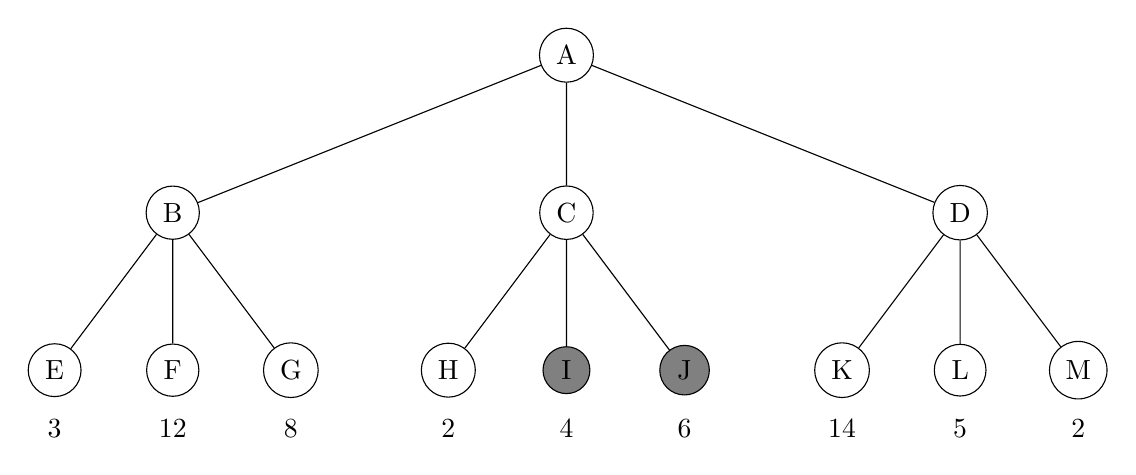
\begin{tikzpicture}[
            level distance=2cm,
            level 1/.style={sibling distance=5cm},
            level 2/.style={sibling distance=1.5cm},
            level 3/.style={sibling distance=1cm}
        ]
        \node[circle,draw] {A}
        child {
                node[circle,draw] (B) {B}
                child {node[circle,draw] (E) {E}}
                child {node[circle,draw] (F) {F}}
                child {node[circle,draw] (G) {G}}
            }
        child {
                node[circle,draw] (C) {C}
                child {node[circle,draw] (H) {H}}
                child {node[circle,draw,fill=gray] (I) {I}}
                child {node[circle,draw,fill=gray] (J) {J}}
            }
        child {
                node[circle,draw] (D) {D}
                child {node[circle,draw] (K) {K}}
                child {node[circle,draw] (L) {L}}
                child {node[circle,draw] (M) {M}}
            };

        \node[below, yshift=-0.5cm] at (E) {3};
        \node[below, yshift=-0.5cm] at (F) {12};
        \node[below, yshift=-0.5cm] at (G) {8};

        \node[below, yshift=-0.5cm] at (H) {2};
        \node[below, yshift=-0.5cm] at (I) {4};
        \node[below, yshift=-0.5cm] at (J) {6};

        \node[below, yshift=-0.5cm] at (K) {14};
        \node[below, yshift=-0.5cm] at (L) {5};
        \node[below, yshift=-0.5cm] at (M) {2};
    \end{tikzpicture}
\end{figure}

因为在对$ B $结点的子树搜索后,将会计算得出MIN在$ B $结点的最小值为$ 3 $。然后在对结点$ C $的搜索中,$ C $的第一个子结点为$ 2 $。由于MIN只会选择其中的最小值,而MAX只会根据这些最小值中的最大值,即:

\vspace{-1cm}

\begin{align*}
    Minimax(root) & = max(min(3, 12, 8), min(2, x, y), min(14, 5, 2)) \\
                  & = max(3, min(2, x, y), 14)                        \\
                  & = 3
\end{align*}

因此Alpha-Beta剪枝在搜索完结点$ H $后,没有必要继续对$ I $和$ J $再进行搜索了。\\

\begin{algorithm}[H]
    \caption{AlphaBetaPruning}
    \begin{algorithmic}[1]
        \Procedure{AlphaBetaSearch}{game, state} returns an action
        \State player = game.ToMove(state)
        \State value, move = MaxValue(game, state, $ -\infty $, $ +\infty $)
        \State \Return move
        \EndProcedure
        \\
        \Procedure{MaxValue}{game, state, $ \alpha $, $ \beta $} returns a (utility, move) pair
        \If {game.IsTermial(state)}
        \State \Return game.Utility(state, player), null
        \EndIf
        \State v = $ - \infty $
        \For {a in game.Actions(state)}
        \State v2, a2 = MinValue(game, game.Result(state, a))
        \If {v2 > v}
        \State v, move = v2, a
        \State $ \alpha $ = max($ \alpha $, v)
        \EndIf
        \If {v >= $ \beta $}
        \State \Return v, move
        \EndIf
        \EndFor
        \State \Return v, move
        \EndProcedure
        \\
        \Procedure{MinValue}{game, state, $ \alpha $, $ \beta $} returns a (utility, move) pair
        \If {game.IsTermial(state)}
        \State \Return game.Utility(state, player), null
        \EndIf
        \State v = $ + \infty $
        \For {a in game.Actions(state)}
        \State v2, a2 = MaxValue(game, game.Result(state, a))
        \If {v2 < v}
        \State v, move = v2, a
        \State $ \beta $ = min($ \beta $, v)
        \EndIf
        \If {v <= $ \alpha $}
        \State \Return v, move
        \EndIf
        \EndFor
        \State \Return v, move
        \EndProcedure
    \end{algorithmic}
\end{algorithm}

\begin{itemize}
    \item 时间复杂度:
          \begin{itemize}
              \item 随机行动顺序:$ O(b^{3m \over 4}) $
              \item 最佳行动顺序(启发式算法):$ O(b^{m \over 2}) $
          \end{itemize}
    \item 空间复杂度:$ O(m) $
    \item 完备性:YES(当博弈树有穷时)
    \item 最优性:YES
\end{itemize}

\newpage